\documentclass[journal]{IEEEtran}
\usepackage[T1]{fontenc}
\usepackage{amsmath,amssymb,booktabs,array,tabularx,url,graphicx}
\usepackage[hidelinks]{hyperref}
\usepackage{microtype}
\newcommand{\FPR}{\operatorname{FPR}}
\newcommand{\BA}{\operatorname{BA}}
\newcommand{\ind}{\mathbf{1}}
\newcommand{\ton}{TON-IoT}
\newcommand{\cic}{CICIoT2023}
\newcommand{\nb}{N-BaIoT}
\hyphenation{data-set data-sets pre-pro-cess-ing}
\makeatletter
\newcommand{\tableinput}[1]{\@@input #1.tex }
\makeatother
% Automatically generated from independent raw-log recomputation.
\newcommand{\RFEnergy}{1206.787}
\newcommand{\RFFOne}{0.983864}
\newcommand{\RFRecallPct}{99.664}
\newcommand{\RFFPRPct}{1.538}
\newcommand{\RFFN}{57.8}
\newcommand{\RFFP}{504.5}
\newcommand{\RFBatchMS}{32.595}
\newcommand{\TQEnergy}{1193.719}
\newcommand{\TQFOne}{0.970439}
\newcommand{\TQRecallPct}{96.710}
\newcommand{\TQFPRPct}{1.364}
\newcommand{\TQFN}{565.9}
\newcommand{\TQFP}{447.5}
\newcommand{\TQBatchMS}{1.447}
\newcommand{\TQSavingJ}{13.068}
\newcommand{\TQSavingJLow}{9.736}
\newcommand{\TQSavingJHigh}{16.400}
\newcommand{\TQSavingPct}{1.082}
\newcommand{\TQFOneDropPP}{1.343}
\newcommand{\TQRecallDropPP}{2.954}
\newcommand{\DQEnergy}{1200.560}
\newcommand{\DQFOne}{0.970439}
\newcommand{\DQRecallPct}{96.710}
\newcommand{\DQFPRPct}{1.364}
\newcommand{\DQFN}{565.9}
\newcommand{\DQFP}{447.5}
\newcommand{\DQBatchMS}{1.482}
\newcommand{\DQSavingJ}{6.227}
\newcommand{\DQSavingJLow}{1.600}
\newcommand{\DQSavingJHigh}{10.853}
\newcommand{\DQSavingPct}{0.515}
\newcommand{\DQFOneDropPP}{1.343}
\newcommand{\DQRecallDropPP}{2.954}
\newcommand{\CFEnergy}{1196.842}
\newcommand{\CFFOne}{0.636440}
\newcommand{\CFRecallPct}{99.335}
\newcommand{\CFFPRPct}{59.164}
\newcommand{\CFFN}{114.4}
\newcommand{\CFFP}{19405.9}
\newcommand{\CFBatchMS}{2.337}
\newcommand{\CFSavingJ}{9.945}
\newcommand{\CFSavingJLow}{7.117}
\newcommand{\CFSavingJHigh}{12.773}
\newcommand{\CFSavingPct}{0.824}
\newcommand{\CFFOneDropPP}{34.742}
\newcommand{\CFRecallDropPP}{0.329}

\begin{document}
\title{When Learned IDS Model Selection Collapses to a Static Choice:\\A Measurement Study at the Edge}
\author{Nuonan~Ouyang,
        Adrian~Shatte,
        Zhigang~Lu,
        Chao~Chen,~\IEEEmembership{Member,~IEEE,}
        and~Wei~Xiang,~\IEEEmembership{Senior Member,~IEEE}%
\thanks{(\textit{Corresponding author: Nuonan Ouyang.})}%
\thanks{N. Ouyang and A. Shatte are with the College of Science and Engineering, Division of Research, James Cook University, Bebegu Yumba Campus, Building 17, Douglas, Townsville, QLD, Australia (e-mail: nuonan.ouyang@my.jcu.edu.au; adrian.shatte@jcu.edu.au; ORCID: 0009-0004-7124-8940; 0000-0002-6225-9697).}%
\thanks{Z. Lu is with the School of Computer, Data and Mathematical Sciences, Western Sydney University, Penrith (Kingswood) Campus, Kingswood, NSW, Australia (e-mail: z.lu@westernsydney.edu.au; ORCID: 0000-0001-5102-6217).}%
\thanks{C. Chen is with the College of Business and Law, RMIT University, Melbourne, VIC 3000, Australia (e-mail: chao.chen@rmit.edu.au; ORCID: 0000-0003-1355-3870).}%
\thanks{W. Xiang is with the Australian Centre for AI in Medical Innovation and the Cisco-La Trobe Centre for AI and Internet of Things, La Trobe University, Melbourne, VIC, Australia (e-mail: w.xiang@latrobe.edu.au; ORCID: 0000-0002-0608-065X).}%
}
\markboth{IEEE Transactions on Network and Service Management,~Vol.~XX, No.~XX, Month~Year}%
{Ouyang \MakeLowercase{\textit{et al.}}: When Learned IDS Model Selection Collapses to a Static Choice}
\maketitle
\begin{abstract}
Learned model selection can appear to save energy when it merely fixes a cheaper detector. On one Raspberry Pi 4B, primary Tabular-Q uses 13.1 J less than Static-MedRF over 500 s (1.08\%; 26.1 mW), but missed-positive presentations rise from 57.8 to 565.9 per 50,000-row replay and the policy selects LightLR throughout. A matched Static-LightLR control resolves no directional Tabular-Q energy difference. We derive a pairwise non-degeneracy test showing that the executed reward scaling requires a 0.7967 balanced-accuracy advantage for MedRF to outrank LightLR before held-out evaluation. Under a prospectively frozen 50/100/4000 rows/s $\times$ 0.10/0.50/0.90 factorial, DeadlineGuard switches between MedRF and LightLR, uses 43.7 J less than Static-MedRF (2.98\%; 95\% paired CI 41.4--46.0 J), and eliminates 512/5,000 deadline misses at a 1.373-pp F1 cost. Frozen DQN remains LightLR, whereas Tabular-Q falls to TinyDT (67.76\% FPR). The results separate detector choice, conditional adaptation, reward specification, and off-support controller behavior in edge IDS orchestration.
\end{abstract}
\begin{IEEEkeywords}
Intrusion detection, IoT, edge resource management, model selection, reinforcement learning, energy measurement, reproducibility.
\end{IEEEkeywords}
\section{Introduction}
Edge intrusion detection must balance attack recognition with latency and energy. Runtime selection appears attractive, but a learned controller may simply choose one detector throughout deployment. Comparing it only with a more expensive static detector then measures an operating-point change rather than adaptive value. In our primary campaign, Tabular-Q saves 13.1 J over roughly 500 s relative to Static-MedRF---1.08\%, or 26.1 mW on average---while missed-positive presentations rise from 57.8 to 565.9 per 50,000-row replay. This scale mismatch motivates a stricter question: \emph{what schedule was actually realized, under what service constraints, and at what security cost?}

We answer that question as a \ton{}-centered systems study with four frozen detectors and paired Raspberry Pi measurements; \cic{} and \nb{} remain supplementary detector/data audits rather than dynamic-power evidence. The evidence separates the primary physical campaign and Static-LightLR attribution control, an analytic reward non-degeneracy screen, and prospectively frozen confidence/deadline-aware controls under fixed and variable load.

Four questions organize the paper: \emph{RQ1}, what security/resource operating points do the frozen \ton{} detectors provide? \emph{RQ2}, do learned selectors improve upon the static schedule they realize, and is their scalar objective non-degenerate on the declared support? \emph{RQ3}, do confidence- and deadline-aware conditional controls provide useful switching? \emph{RQ4}, how do state coverage, off-support actions, deadline violations, and threshold calibration constrain deployment claims?

Our contributions are: (i) paired whole-device evidence that places a small resource effect beside its much larger missed-detection cost; (ii) a pairwise non-degeneracy criterion that converts reward weights and normalization into a pre-deployment preference-reversal test; (iii) static, learned, confidence-cascade, and variable-load controls that separate detector choice from conditional orchestration; and (iv) an off-support failure analysis showing how sparse discrete-state coverage can expose unsafe default actions. Together, the study identifies when learned IDS orchestration does---and does not---realize adaptive service value.

\begin{figure*}[t]
\centering
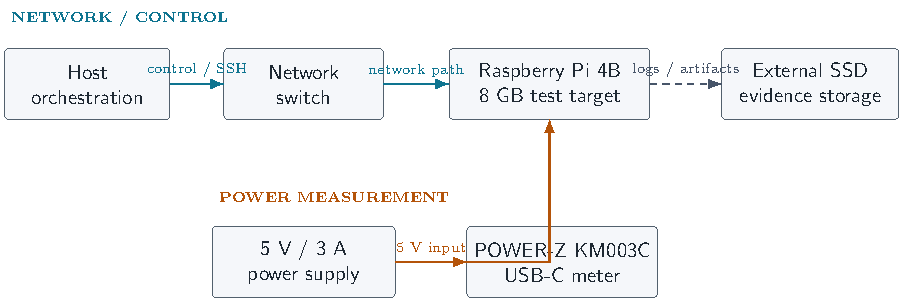
\includegraphics[width=.82\textwidth]{figures/experiment_setup_schematic.pdf}
\caption{Schematic apparatus overview. Network orchestration reaches the Raspberry Pi 4B through the switch, while the 5-V supply feeds the Pi through the KM003C meter; the external SSD stores evidence artifacts. The drawing identifies roles and paths only and contains no synthetic measurement readout.}
\label{fig:experimentdesign}
\end{figure*}

\section{Related Work and Evaluation Perspective}
\subsection{Dynamic IDS Selection and Conditional Inference}
Recent IDS work spans continual/incremental detection, heterogeneous representations, and runtime model selection~\cite{Wang2024BFSNID,AOCIDS2024,StatAvg2025,DMIDS2025}. Our detector artifacts are frozen; the runtime problem is which detector to execute. Auto-IDaS uses DQN for detector selection under traffic variation, whereas FEDMS uses confidence-driven dynamic selection~\cite{Lin2024AutoIDaS,Hasan2026FEDMS}. These establish plausible adaptive mechanisms, but not that a learned selector provides value beyond the static action it realizes.

Conditional computation provides a direct non-RL alternative. BranchyNet, adaptive network selection, MSDNet, and shallow--deep networks use confidence or budget signals to invoke more computation only for harder inputs~\cite{Teerapittayanon2016BranchyNet,Bolukbasi2017Adaptive,Huang2018MSDNet,Kaya2019ShallowDeep}. At the serving layer, Clipper, INFaaS, and Clockwork expose accuracy/latency/cost trade-offs and request-level SLOs~\cite{Crankshaw2017Clipper,Romero2021INFaaS,Gujarati2020Clockwork}. These motivate our confidence cascade and deadline-aware comparator.

\subsection{Learned Resource Orchestration and Evaluation}
Reinforcement learning is widely used for runtime resource orchestration. TNSM examples include measurement-informed vRAN reconfiguration and vehicle--edge scheduling~\cite{Murti2024vRAN,Zhang2024VehicleEdge}; related mobile/edge systems couple DVFS, dependent-task scheduling, offloading, and QoS control to latency or energy objectives~\cite{Zhang2024DVFO,Lou2024Startup,Kim2024DistributedOffload,Maleki2024QCS,Nan2026RobustDNN,Wang2025TrustOffload,Hu2025SITOff,Zhang2024AoI,Luo2025SolarEdge}. Tabular Q-learning estimates values in a discrete state space~\cite{Watkins1992}, while DQN uses a neural action-value approximator~\cite{Mnih2015}. Controller complexity, however, is not evidence of useful adaptation.

Security-ML evaluations can be optimistic even when implementations are internally correct~\cite{Arp2022}. We therefore expose source/encoded-data identity, confusion counts, realized actions, deadlines, and raw meter frames, and keep training variability, replay resampling, and physical repeatability as separate uncertainty sources~\cite{Agarwal2021}. The block---not rows, windows, or meter samples---is the physical repeat unit.

\section{Dataset-Native Data Preparation}
The main systems study uses \ton{}. Its frozen pipeline retains 32 native features and admits no feature into a cross-dataset core. The \ton{} split groups unordered IP pairs, fits imputation/scaling/categorical encoding on training data only, and uses training seed 11. Source-row identifiers and raw-field fingerprints are cross-partition disjoint; the independent encoded-float32 audit finds zero \ton{} train--test vector matches. Exact counts, lineage, and split membership are supplementary.

The same ledger also records dataset-native \cic{} and \nb{} pipelines (39 and 115 native features), but these are supplementary detector/data audits only. Their coverage and encoded-overlap limitations are retained rather than used to imply cross-dataset dynamic-power generality~\cite{CICSource}.

\section{Frozen Detectors and Causal Scheduling}
\subsection{Detector Pool}
Each dataset has four separately fitted configurations: depth-6 TinyDT; L2 LightLR; 25-tree, depth-10 MedRF; and a 64/32/16 HeavyMLP. All use threshold 0.5 and training seed 11. Names do not assert a resource ranking. During \ton{} physical experiments all models remain resident; an action selects one model for the next batch without loading, fitting, or updating it.

\subsection{Decision Information and State Encoding}
Before window $t$, the controller constructs
\begin{equation}
 s_t=(\widetilde T_t,h_{t-1},q_t,\lambda_{t-1},a_{t-1}).
\end{equation}
The kernel temperature is smoothed as $\widetilde T_t=0.9\widetilde T_{t-1}+0.1T_t$, initialized at $T_0$. The threat observation $h_{t-1}$ is the arithmetic mean attack probability from the single detector selected in the preceding window; it is not the preceding ground-truth attack fraction. Queue utilization is bounded to $[0,1]$, and the preceding arrival count is divided by 100 and bounded to $[0,2]$. Initial threat, arrival ratio, and preceding action are 0.5, 1, and TinyDT.

Each of the first four state variables has three bins. Their two boundaries are $(45,70)$ degrees Celsius, $(1/3,0.7)$ for threat, $(1/3,2/3)$ for queue utilization, and $(0.9,1.1)$ for arrival ratio. Including four previous actions gives $3^4\times4=324$ states. Boundary equality enters the higher bin. The flat index is row-major in this listed order, with previous action changing fastest.

The executed order is state, committed/logged action, selected-model inference, outcome log, then lagged-state update. Ground truth, cell identity, and unselected current-window outputs are unavailable online. Original software traces use 35$^\circ$C, zero queue, and 100 arrivals/window; the variable-load experiment varies causal arrival count and prevalence without revealing factorial-cell identity.

\subsection{Reward and Cost Provenance}
The unchanged per-window training reward is
\begin{equation}\label{eq:reward}
 r_t=0.5B_t-0.2\overline P_t-0.2\overline L_t-0.1\overline H_t,
\end{equation}
where $B_t$ is balanced accuracy over classes present in the window. All evaluated phase windows contain both classes. With $[x]_0^1=\min(1,\max(0,x))$, the normalization is
\begin{align}
 \overline P_t&=\left[\frac{P_t-2.347219336}{0.049806200}\right]_0^1,\\
 \overline L_t&=\left[\frac{L_t-1.2979595}{29.6547998}\right]_0^1,\\
 \overline H_t&=\left[\frac{\max(0,T_t^{\rm post}-\widetilde T_t)}{1\,{}^\circ\mathrm C}\right]_0^1.
\end{align}
$P_t$ and $L_t$ are frozen \ton{} paced-profile lookups, not contemporaneous training measurements. Their means are 2.353132/1.297960, 2.347219/1.544420, 2.397026/30.952759, and 2.366688/4.417836 W/ms for TinyDT, LightLR, MedRF, and HeavyMLP. No fitted thermal response or switching-energy penalty is used.

\subsection{Pre-deployment Pairwise Non-degeneracy Check}
The scalar objective can be screened before policy evaluation. For two actions $a,b$, let $D_a(s)$ denote the detection term and let $C_a=\sum_j w_j\bar C_{j,a}$ collect normalized resource penalties that are fixed on the declared support (as in the executed training profiles at neutral thermal cost). Then
\begin{equation}
 U_a(s)-U_b(s)=w_D\Delta D_{ab}(s)-\Delta C_{ab},\qquad
 \tau_{ab}=\frac{\Delta C_{ab}}{w_D}.
\end{equation}
A strict pairwise preference reversal is possible on support $\mathcal S$ iff
\begin{equation}\label{eq:nondeg}
 \min_{s\in\mathcal S}\Delta D_{ab}(s)<\tau_{ab}<\max_{s\in\mathcal S}\Delta D_{ab}(s).
\end{equation}
If $\tau_{ab}$ lies outside this attainable interval, no optimizer can make the pair exchange rank under the frozen scalar utility on that support. For MedRF versus LightLR, the declared min--max scaling gives $\tau=0.7967$: an almost 80-percentage-point balanced-accuracy advantage would be required to offset the frozen nonthermal resource penalty. This threshold is determined only by the declared weights and resource profiles and can therefore be inspected before held-out evaluation; whether reversal is attainable is then checked against calibration/validation support rather than test outcomes. Candidate-pool min--max denominators make this exchange rate change whenever pool membership changes. For deployment, external denominators such as idle-relative power budgets, latency SLOs, or thermal headroom preserve a physically interpretable exchange rate. The proof and numerical decomposition are supplementary.

\subsection{Policies and Offline Selection}
CFSM is a fixed heuristic initialized to TinyDT. At a smoothed temperature of at least 70 degrees it steps down one model rank, bypassing cooldown. Otherwise it holds for two complete windows after a switch; when no cooldown remains, threat below 0.7 steps down one rank and threat at least 0.7 steps up one rank. Boundary actions hold. Queue and load are logged but not used by CFSM. This fixed ordering is evaluated as implemented, not asserted to be optimal.

Tabular-Q uses zero initialization, learning rate 0.1, discount 0.9, and the update
\begin{equation}
 \begin{aligned}
 Q(s_t,a_t)&\leftarrow Q(s_t,a_t)+0.1\delta_t,\\
 \delta_t&=r_t+0.9\max_aQ(s_{t+1},a)-Q(s_t,a_t),
\end{aligned}
\end{equation}
with zero terminal bootstrap~\cite{Watkins1992}. DQN uses one-hot state, two 64-unit ReLU layers, Adam 0.001, replay 10,000, batch 32, and a target copy every 250 updates~\cite{Mnih2015}. Both train for 1,000 episodes with epsilon 1 to 0.01. Checkpoints are selected every 25 episodes on five validation traces; test execution freezes the policy and performs no update. Full training, tie rules, seeds, and later multi-seed/sensitivity results appear in the supplement.

\section{Completed Evaluation and Measurement Methods}
\subsection{Classification and Static Evidence}
The held-out classification evaluation uses the frozen threshold and reports attack-class F1, recall, balanced accuracy, false-positive rate, and the full confusion counts. In particular,
\begin{align}
 \FPR &= \frac{FP}{TN+FP},\\
 \BA &= \tfrac12\left(\frac{TP}{TP+FN}+\frac{TN}{TN+FP}\right),\\
 F1 &= \frac{2TP}{2TP+FP+FN}.
\end{align}
Counts are pooled over the declared evaluation unit before metrics are calculated. The supplement retains 50 static traces and 200 model--trace evaluations. These reuse fixed held-out pools and do not constitute fresh attacks, classifier retraining, or physical repeats.

\subsection{Pi Prediction Consistency and Inference Timing}
Pi parity checks cover 12 dataset--model combinations and 10,000 encoded rows each with zero threshold-label disagreements. Tight-loop timing reports 100-row inference after warm-up and excludes encoding, transport, queueing, and controller cost.

\subsection{Static Whole-Device Power}
The physical reference uses one Pi 4B 8 GB and inline POWER-Z KM003C. Fifteen valid 1,800-second segments comprise three repeats of instrumented idle and four \ton{} detectors, all resident, at 100 preencoded rows/s. This is resource characterization, not another detection test.

The meter records nominally 1 Hz boundary samples, including raw ADC replies, signed current, voltage, and monotonic request/receive times. Under the recorded connector orientation, consumed power is calculated as $P_i=V_i(-I_i)$. Using the observed sampling times $\tau_i$, input energy is approximated by
\begin{equation}
 E=\sum_{i=1}^{n-1}\frac{P_i+P_{i+1}}{2}(\tau_{i+1}-\tau_i),
 \qquad \bar P=\frac{E}{\tau_n-\tau_1}.
\end{equation}
No missing sample is filled. This is 1-Hz load-side USB energy, not calibrated wall-side measurement or a subsecond waveform.

\subsection{Statistical Units and Interval Reporting}
For an outcome $z$ observed over $n$ declared repetitions, the two-sided interval is
\begin{equation}\label{eq:tci}
 \bar z \pm t_{0.975,n-1}\frac{s_z}{\sqrt n},
\end{equation}
using the sample SD~\cite{NISTMean}. Physical scheduler inference uses ten paired blocks, never rows, windows, or meter frames. Raw energy is primary. Drift sensitivity subtracts each run's preceding idle power; it is reported separately rather than substituted for raw measurement. Exact $2^{10}$ sign-flip tests are secondary diagnostics.

\subsection{Physical Campaigns}
The primary campaign contains ten matched 500-second blocks of Static-MedRF, CFSM, Tabular-Q, and DQN. matched-control subsequently adds ten blocks with the missing Static-LightLR control; scheduler-overhead isolates state-to-action timing; multi-seed--hyperparameter sensitivity test seeds, reward/state variants, and Tabular-Q $\alpha/\gamma$. They do not replace the frozen primary policy.

A fixed-rate confidence-cascade control uses ten new matched blocks at 100 rows/s with Static-LightLR, a fixed confidence cascade, frozen Tabular-Q, and Static-MedRF. The cascade first runs LightLR and escalates a row to MedRF iff LightLR attack probability is in the fixed band $[0.3,0.7]$.

A variable-load campaign uses ten blocks and six methods over 500 seconds. Each run visits the nine predeclared 50-second cells $\{50,100,4000\}$ rows/s $\times\{0.10,0.50,0.90\}$ attack prevalence exactly once, followed by 50 seconds at 100/0.10. DeadlineGuard uses only current causal arrival count: MedRF is chosen when $\lceil N/100\rceil L_{95}^{\rm RF}\le1$ s, otherwise LightLR. The threshold and workload were frozen from previously measured latency. Completion timestamps define a one-second service deadline; queue, states, actions, fallbacks, and misses are retained.

controller-only power arm predeclared controller-only physical power over four ``original observed-support states.'' The frozen artifact contains eight such states and no rule uniquely identifies four; under the stop rule controller-only power arm is \texttt{NOT\_EXECUTED}. TinyDT threshold diagnostic chooses a TinyDT threshold on validation by maximum balanced accuracy (highest-threshold tie break), hashes it, and applies it once to test. This diagnostic never replaces threshold 0.5.

\section{Completed Static Results}
\subsection{TON-IoT Detection Operating Points}
Table~\ref{tab:classification} shows the four \ton{} operating points used by the physical study. TinyDT has recall 0.9976 but F1 0.4792 and FPR 67.78\%; LightLR, MedRF, and HeavyMLP have F1 0.9620--0.9746 and FPR 1.35--1.52\%. Full confusion counts, plus \cic{}/\nb{} detector and overlap audits, are retained in the supplement rather than used to imply cross-dataset dynamic-power generality.

\begin{table}[t]
\centering\small
\caption{TON-IoT held-out detection at threshold 0.5. BA denotes balanced accuracy; FPR is a percentage.}
\label{tab:classification}
\setlength{\tabcolsep}{4.2pt}
\begin{tabular}{lrrrr}\toprule
Model & F1 & Recall & BA & FPR (\%)\\\midrule
\tableinput{tables/ton_classification_rows}
\bottomrule\end{tabular}
\end{table}

For attack prevalence $p$, recall $r$, and FPR $f$,
\begin{equation}\label{eq:prevalence}
 F1=\frac{2pr}{p(1+r)+(1-p)f},
\end{equation}
so high attack prevalence can coexist with high F1 and poor normal-class behavior. Static replay and encoded-overlap diagnostics are supplementary and do not change the fixed split, model, or primary threshold.

\subsection{Static Physical Resource Measurements}
Across fifteen static segments, idle averages 2.335 W and active means span 2.347 W (LightLR) to 2.397 W (MedRF). MedRF's paired increment is 61.6 mW [32.1,91.0]; TinyDT and LightLR intervals cross zero. No accepted workload window records undervoltage or throttling. Full segment statistics are supplementary; labels such as ``Tiny'' or ``Heavy'' are not used as empirical cost ranks.

\section{Physical Scheduler Results}
\subsection{Primary Attribution and Robustness}
All forty primary runs contain 501 power samples and 500 decisions. Relative to Static-MedRF, Tabular-Q saves \TQSavingJ{} J (95\% paired CI \TQSavingJLow{}--\TQSavingJHigh{}) and DQN saves \DQSavingJ{} J (\DQSavingJLow{}--\DQSavingJHigh{}), but both lose \TQFOneDropPP{} F1 pp and \TQRecallDropPP{} recall pp. Both select LightLR in all 5,000 windows; thus the result does not demonstrate switching.

The matched Static-LightLR control directly compares the learned policies with Static-LightLR. Tabular-Q has identical predictions and +0.455 J with CI $[-1.861,2.772]$ J; DQN has identical predictions and +4.525 J [2.693,6.357]. The isolated state-to-action benchmark time is 10.8~$\mu$s for Tabular-Q and 1.567 ms for DQN, but timing is not converted into joules. Twenty policy seeds, 85 reward/state runs, and 35 Tabular-Q $\alpha/\gamma$ runs remain single-action on held-out support; only the detection-only objective selects MedRF rather than LightLR. Full primary and strengthening tables are supplementary.

\subsection{Fixed-Rate Confidence Cascade}
Table~\ref{tab:r1} reports ten new matched blocks. The fixed cascade escalates 1.34\% of rows and raises F1 by 1.347 pp versus Static-LightLR while using +7.952 J [5.897,10.007]. Its raw mean-power difference is +15.917 mW [11.798,20.035], whereas preceding-idle adjustment gives +13.635 mW $[-1.515,28.784]$; environmental drift therefore weakens the power attribution but not the raw-energy result. Cascade F1 (0.98391) is close to Static-MedRF (0.98386), with 0.279 lower recall pp and 0.156 lower FPR pp.

The cascade latency is implementation- and call-granularity-specific. Frozen executed source first runs LightLR on the full 100-row batch and, when needed, makes \emph{one} MedRF call on the deferred sub-batch; it does not call MedRF once per deferred row. Although only 1.3388\% of rows are deferred, they are spread across 3,338/5,000 windows (66.76\%), with only 2.01 deferred rows per active window. Windows without escalation average 1.636 ms, whereas escalation-active windows average 31.884 ms, close to the cost of one MedRF call; the resulting overall cascade mean is 21.830 ms. Thus This campaign measures this 100-row, small-sub-batch implementation regime and is not a general energy or latency bound for optimized cascade systems.

\begin{table*}[t]
\centering\footnotesize
\caption{Fixed-rate cascade physical results; means over ten paired blocks. Adjusted power subtracts the immediately preceding idle. Escalation is the fraction sent from LightLR to MedRF.}
\label{tab:r1}
\setlength{\tabcolsep}{4.0pt}
\begin{tabular}{lrrrrrrr}\toprule
Method & Energy (J) & Power (W) & Adjusted (mW) & F1 & Recall (\%) & FPR (\%) & Escalation (\%)\\\midrule
\tableinput{tables/r1_revision_rows}
\bottomrule\end{tabular}
\end{table*}

\subsection{Variable Load, Feasibility, and State Coverage}
The variable-load campaign visits all nine frozen load/prevalence cells in every run. DeadlineGuard executes MedRF in 3,500 and LightLR in 1,500 of its 5,000 windows, with 5.3 recorded switches/run, and misses no service deadline. Static-MedRF misses 512/5,000 deadlines (10.24\%, block CI 9.32--11.16\%) although its final backlog returns to zero. Cascade misses 21/5,000; all other methods miss none.

The strongest paired comparison is DeadlineGuard against Static-MedRF. DeadlineGuard uses 43.714 J less per run (95\% paired CI 41.418--46.010 J), a 2.98\% reduction relative to the 1468.1-J Static-MedRF mean, while reducing the deadline-miss rate by 10.24 pp to zero. The trade-off is 1.373 pp lower F1 and 2.853 pp lower recall. All ten energy differences have the same direction (exact sign-flip $p=0.00195$). This establishes a measured feasibility/energy benefit for the simple causal rule relative to the high-security static baseline, not universal superiority over all static choices.

The frozen learned policies do not provide useful load adaptation. DQN remains LightLR in all 5,000 windows and reproduces its detection. Tabular-Q reaches new load-related states and selects TinyDT in every window through the frozen tabular default, yielding F1 0.7434 with FPR 67.76\%. Here ``fallback'' is registry terminology, not an exception branch. On unseen zero-initialized rows, \texttt{np.argmax} returns the first maximum and the configured action order places TinyDT first. Thus the variable-load failure is the hardware realization of the off-support tie behavior already visible in the 314/324-state TinyDT greedy map.

The fixed heuristic provides a switching contrast rather than a no-op baseline. CFSM averages 9.8 switches per run, but spends 74.20\% of windows on TinyDT and only 22.26\% on HeavyMLP (LightLR 2.28\%, MedRF 1.26\%). Its switching changes detector identity without reaching a reliable security operating point; the low F1 is not evidence that CFSM simply selected one static model.

Variable-load raw energy is heterogeneous across methods, so Table~\ref{tab:r2} now reports run SDs and selected paired contrasts are separated in Table~\ref{tab:r2pairs}. For DQN versus Static-LightLR, all ten raw block differences are positive (median +5.72 J; exact sign-flip $p=0.00195$), but one Block~4 excursion is +392.0 J and inflates the SD of differences to 122.2 J, giving a Student-$t$ interval of $[-43.2,131.7]$ J. That run coincides with a 3.919-W preceding idle and a 49.2$^\circ$C maximum temperature, unlike the other DQN blocks; idle-adjusted power does not resolve a DQN--LightLR difference. We therefore report a consistent raw direction but an unstable magnitude and make no controller-power attribution because the controller-only power arm was not executed.

For scale only, the isolated DQN state-to-action timing is 1.5669~ms. Five thousand decisions therefore amount to 7.8345~s of controller CPU time. If an external device-power increment were hypothetically 0.2, 0.5, or 1.0~W, the corresponding upper-bound contributions would be 1.57, 3.92, and 7.83~J, respectively. These are sensitivity calculations, not measurements: no controller-power increment was measured and none is used to attribute the physical DQN premium.

DeadlineGuard uses +7.550 J [5.033,10.068] and +14.160 adjusted mW [0.374,27.947] relative to Static-LightLR. Static-MedRF uses +51.264 J [49.537,52.991] and +98.609 adjusted mW [79.296,117.922] relative to LightLR. Cascade improves F1 by 1.384 pp but its raw +31.262 J interval crosses zero; the idle-adjusted +98.843 mW interval [77.885,119.802] does not. Raw and preceding-idle-adjusted endpoints are retained separately because they answer different questions.

\begin{table*}[t]
\centering\footnotesize
\caption{Variable-load results over ten paired blocks. Energy is mean$\pm$SD across runs; deadline miss is the fraction of one-second windows missing the service deadline.}
\label{tab:r2}
\setlength{\tabcolsep}{3.1pt}
\begin{tabular}{lrrrrrrr}\toprule
Method & Energy (J) & Power (W) & F1 & Recall (\%) & FPR (\%) & Miss (\%) & Completion p95 (s)\\\midrule
\tableinput{tables/r2_revision_rows}
\bottomrule\end{tabular}
\end{table*}

\begin{table}[t]
\centering\scriptsize
\caption{Selected variable-load paired contrasts, $n=10$ blocks. $\Delta E$ is first method minus second; detection and deadline changes are percentage points.}
\label{tab:r2pairs}
\resizebox{\columnwidth}{!}{%
\begin{tabular}{lrrrr}\toprule
Contrast & $\Delta E$ (J), 95\% CI & $\Delta$F1 & $\Delta$Miss & sign-flip $p$\\\midrule
\tableinput{tables/r2_key_paired_rows}
\bottomrule\end{tabular}}
\end{table}

\begin{figure}[t]
\centering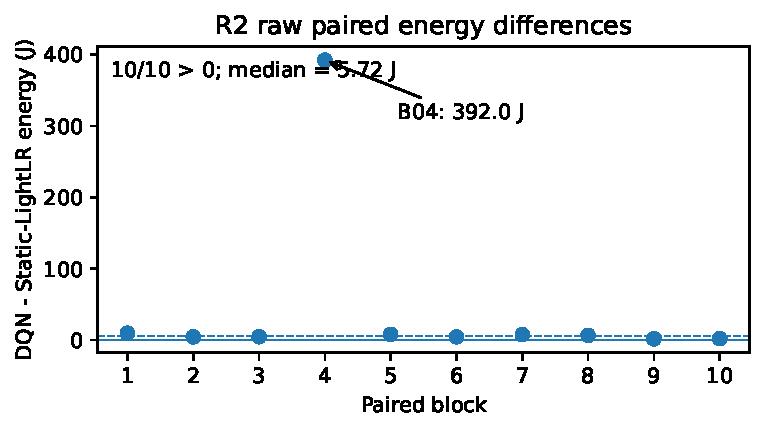
\includegraphics[width=\columnwidth]{figures/r2_dqn_block_energy_differences.pdf}
\caption{Raw DQN-minus-Static-LightLR energy difference for each paired block. All ten are positive, but Block~4 is a large power/temperature excursion; the dashed line is the median (5.72 J).}
\label{fig:r2dqnblocks}
\end{figure}

\begin{figure}[t]
\centering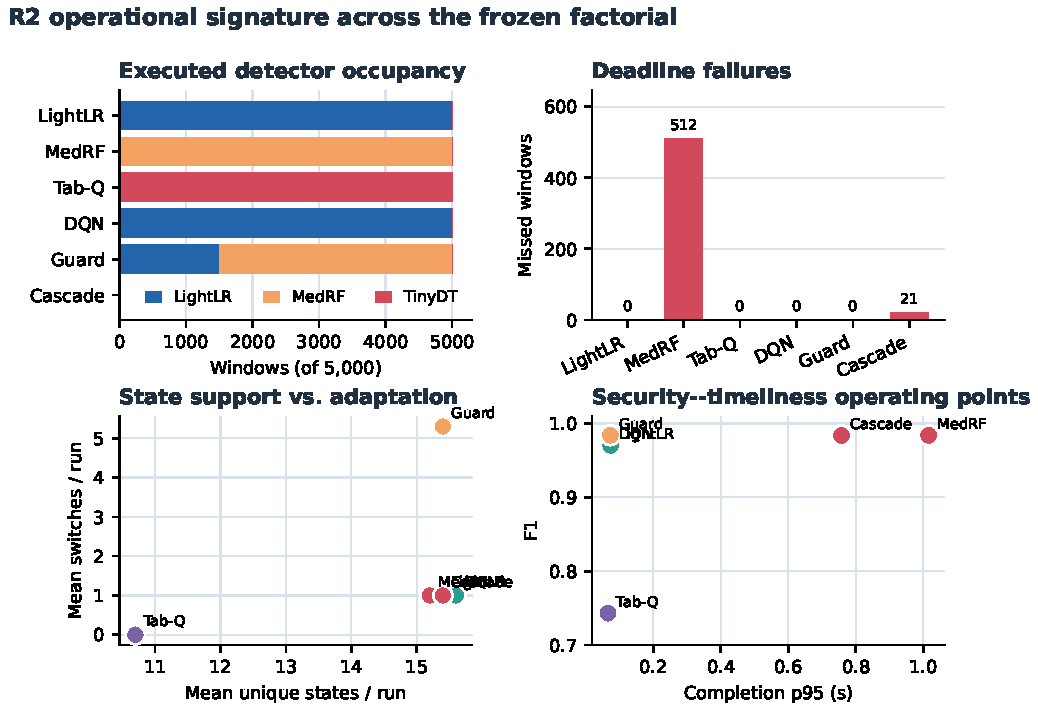
\includegraphics[width=\columnwidth]{figures/r2_operational_dashboard.pdf}
\caption{Variable-load operational dashboard: realized detector occupancy, deadline misses, state support/switching, and security--timeliness operating points in the same frozen 60-run factorial.}
\label{fig:r2dashboard}
\end{figure}

\subsection{Protocol Stop and TinyDT Threshold Diagnostic}
The planned controller-only power arm is not missing data: it is a protocol-preserving stop. Its design required four original observed-support states, but the frozen registry exposes eight and supplies no pre-outcome selection rule. Choosing four afterward would modify the protocol, so no controller-only power segment was run and no DQN joule attribution is made.

The threshold diagnostic selects threshold 0.646751 on validation and applies it once to test. At threshold 0.5, TinyDT test F1/FPR/recall are 0.4792/67.78\%/99.76\%; the diagnostic yields 0.9698/1.82\%/99.61\%, with balanced accuracy 0.9889 and AUROC 0.9906. The large recovery with near-constant recall is consistent with a shifted decision threshold rather than absent ranking information. It does \emph{not} make TinyDT an acceptable substitute in the frozen physical study: every classifier and scheduler artifact in those campaigns was fixed at threshold 0.5, and the post-hoc threshold cannot retroactively rehabilitate the unsafe TinyDT actions. The diagnostic therefore explains calibration sensitivity without replacing any primary or physical result.

\begin{table}[t]
\centering\scriptsize
\caption{TON-IoT TinyDT test: fixed primary versus post-hoc validation-selected threshold.}
\label{tab:r4}
\setlength{\tabcolsep}{2.1pt}
\resizebox{\columnwidth}{!}{%
\begin{tabular}{lrrrrrrrrr}\toprule
Result & $\tau$ & TN & FP & FN & TP & F1 & Rec. & FPR & BA\\\midrule
\tableinput{tables/r4_threshold_rows}
\bottomrule\end{tabular}}
\end{table}

The same validation-only procedure was also applied offline to the other frozen TON-IoT detector scores. Table~\ref{tab:allthreshold} shows the resulting test diagnostics; no detector was retrained and no physical campaign was changed. TinyDT is the clear F1/FPR outlier: its validation-selected threshold changes test F1 by +49.05 points, whereas the other detectors change by at most 0.29 points. This separates calibration sensitivity from the sparse-state and deterministic-tie mechanism.

\begin{table*}[t]
\centering
\footnotesize
\caption{Offline validation-selected threshold diagnostic for every frozen TON-IoT detector. The physical campaigns remain fixed at $\tau=0.5$.}
\label{tab:allthreshold}
\setlength{\tabcolsep}{4pt}
\begin{tabular}{lrrrrrrr}\toprule
Model & $\tau=0.5$ F1 & $\tau=0.5$ FPR (\%) & $\tau^\star$ & $\tau^\star$ F1 & $\tau^\star$ FPR (\%) & $\Delta$F1 (pp) & Validation BA\\\midrule
\tableinput{tables/all_detector_threshold_rows}
\bottomrule\end{tabular}
\end{table*}

\section{Discussion}
\subsection{Attribution, Adaptation, and Operational Scale}
The primary learned energy reduction is mainly detector choice: both learned policies execute LightLR, and the matched control resolves no Tabular-Q saving or premium against direct LightLR. Its 13.1 J contrast with Static-MedRF is only 26.1 mW on average while missed-positive presentations increase almost tenfold. At the primary 100 rows/s cadence, detector inference occupies only a small fraction of each one-second interval, so background platform power dominates the whole-device endpoint. Energy alone would therefore overstate the practical value of the learned policy.

The variable-load campaign supplies the positive service-management result that the primary campaign lacked. Relative to Static-MedRF, DeadlineGuard reduces energy by 43.7 J per run (2.98\%; 95\% paired CI 41.4--46.0 J) and eliminates a 10.24-pp deadline-miss rate, at a 1.373-pp F1 cost. Unlike the learned selectors, it realizes load-conditioned switching under the prospectively frozen factorial. This does not make DeadlineGuard universally optimal: Static-LightLR is still lower-energy and has the same zero deadline misses, while DeadlineGuard trades +7.55 J for a small 0.056-pp F1 gain relative to LightLR. The value of the comparison is that the high-security static baseline becomes infeasible at the declared service deadline and a simple causal rule exposes that trade-off explicitly.

The confidence cascade answers a different question. It recovers MedRF-like F1 using only 1.34\% row escalation, but those rows occur in 66.76\% of 100-row windows. The executed implementation performs one MedRF call per escalation-active window on a tiny deferred sub-batch, and that call has near-MedRF latency. Its observed whole-device cost is therefore specific to this call granularity and should not be read as a general limit on optimized batched cascades.

\subsection{Reward Specification as a Pre-deployment Check}
The policy collapse is not only an empirical observation. Equation~\eqref{eq:nondeg} exposes whether the frozen scalar utility even permits a pair of actions to exchange rank on the declared support. For MedRF versus LightLR, candidate-range normalization implies a 0.7967 balanced-accuracy threshold---an almost 80-percentage-point exchange rate determined before held-out evaluation. A controller can therefore appear to ``learn'' a stable choice even when the declared objective makes reversal implausibly demanding on its calibration/validation support. The broader design lesson is to normalize resource terms against deployment contracts---idle-relative power, latency SLOs, energy budgets, or thermal headroom---rather than the arbitrary extrema of the current candidate pool.

\subsection{Sparse Support and Off-support Safety}
Tabular-Q's full greedy map assigns 314/324 states to TinyDT and only ten to LightLR, while formal primary execution reaches four LightLR states. Frozen source confirms that this is not a separate runtime-exception fallback: unseen zero-initialized Q rows are tied, \texttt{np.argmax} returns the first maximum, and TinyDT is action index zero. variable-load campaign makes the consequence concrete: new load-related states drive the frozen table to TinyDT, increasing FPR by roughly 66 percentage points versus LightLR. The transferable risk is therefore the interaction of sparse support, unsafe default action ordering, and deterministic tie breaking. DQN maps the primary 324-state grid to LightLR, but that smoother off-support behavior is not evidence of validated generalization. A deployable discrete controller should report state coverage, the full action map, and the safety quality of unvisited/default actions---not only occupancy on visited states.

\subsection{Measurement and Evaluation Implications}
The variable-load campaign also illustrates why raw means alone are insufficient at small whole-device effects. DQN executes LightLR in every window, yet its raw energy difference from Static-LightLR is positive in 10/10 blocks while the Student-$t$ interval crosses zero because one thermal/power excursion dominates the variance. Reporting the block points, SD, median, exact sign-flip sensitivity, and preceding-idle adjustment exposes this instability; none licenses a causal controller-power explanation because the controller-only power study stopped before measurement.

A learned orchestrator should therefore be compared with the static action it realizes and with simple conditional controls when workload feasibility changes. Action occupancy, deadline violations, and confusion counts are indispensable: energy alone would favor the failed TinyDT collapse, while F1 alone would hide false alarms and service infeasibility. Raw and idle-adjusted physical endpoints answer different questions and neither is selected post hoc because it looks favorable.

The TinyDT diagnostic shows that its threshold-0.5 failure is substantially calibration-sensitive. That does not legitimize replacing the primary threshold after test inspection or treating TinyDT as safe in the already frozen physical campaigns. It instead motivates validation-only calibration governance before deployment. Generalization beyond this operating envelope still requires untouched traffic, additional boards, and independent metrology.

\section{Limitations and Reproducibility Boundary}
Classifier results use one training seed, dataset-native fixed splits, and threshold 0.5. Replay reuses held-out pools. Only \ton{} receives dynamic physical testing; \cic{} and \nb{} provide classification/replay evidence. Ten blocks on one Pi do not estimate board, meter, site, or fleet variability.

The KM003C is not laboratory calibrated; 1-Hz load-side USB measurements exclude AC conversion, network capture, and feature encoding. Models remain resident, temperatures stay low, and the factorial is scheduled feature replay rather than live packet arrival. Pairing reduces but cannot remove ambient drift, as the raw and preceding-idle-adjusted comparisons demonstrate. DQN raw energy in the variable-load campaign is highly skewed by one block with elevated preceding idle power and temperature; the direction is reported separately from the unstable magnitude. The fixed-rate cascade cost is specific to a 100-row windowing regime in which sparse deferred rows trigger a near-fixed-cost MedRF sub-batch call in 66.76\% of windows.

The matched-control, overhead, and sensitivity analyses and the TinyDT threshold diagnostic are post-hoc to the primary campaign. The fixed-rate cascade and variable-load campaigns were prospectively frozen for their own execution. No equivalence margin was declared. The planned controller-only power study supplies no controller-power number because the frozen four-state selection was ambiguous. The TinyDT threshold diagnostic assesses threshold sensitivity without replacing the fixed result. Invalid attempts and replacements remain archived; manifests, CRC, source hashes, and leakage validators establish package integrity, not external validity.

\section{Conclusion}
The experiments separate adaptive value from detector choice and controller implementation. Primary Tabular-Q appears cheaper than Static-MedRF only because it fixes LightLR; under expanded load, the same frozen table falls to a TinyDT default with 67.76\% FPR, while DQN remains LightLR. In contrast, the simple causal DeadlineGuard switches between MedRF and LightLR, uses 43.7 J less than Static-MedRF (2.98\%), and removes all 512 measured deadline misses at a 1.373-pp F1 cost. The pairwise non-degeneracy test explains how reward normalization can suppress action reversal before deployment, and the off-support analysis shows how zero-initialized tabular ties can expose an unsafe default action. Learned IDS orchestration should therefore be credited with adaptive value only after realized actions, relevant static and conditional controls, service feasibility, security loss, and whole-device cost are separated.

\bibliographystyle{IEEEtran}
\bibliography{references}
\end{document}
